\documentclass[12pt]{beamer}
\geometry{paperwidth=254mm,paperheight=190.5mm}
\usepackage{amsmath,amssymb,bm,graphicx,type1cm}
\usefonttheme{serif}
\setbeamersize{text margin left=10mm,text margin right=10mm}
\definecolor{ink}{RGB}{28,48,67}
\definecolor{muted}{RGB}{90,102,114}
\setbeamercolor{normal text}{fg=black,bg=white}
\setbeamercolor{frametitle}{fg=ink}
\setbeamercolor{structure}{fg=ink}
\setbeamerfont{frametitle}{size=\fontsize{18}{22}\selectfont}
\setbeamertemplate{navigation symbols}{}
\setbeamertemplate{frametitle}{\vspace{3mm}\insertframetitle\par\vspace{2mm}\hrule\vspace{1mm}}
\setbeamertemplate{footline}{\hspace{10mm}\color{muted}\fontsize{8}{10}\selectfont Chiral Domain Wall Modes in Adaptive Quantum Dynamics\hfill 7 October 2026\hspace{6mm}\insertframenumber/\inserttotalframenumber\hspace{10mm}\vspace{4mm}}
\newcommand{\bfr}{\boldsymbol r}
\newcommand{\mc}[1]{\mathcal{#1}}
\newcommand{\mr}[1]{\mathrm{#1}}
\newcommand{\Id}{\mathbf{1}}
\hypersetup{pdftitle={Chiral Domain Wall Modes in Adaptive Quantum Dynamics: Figure Overview},pdfsubject={All 14 manuscript figures with captions},pdfauthor={}}
\title{Chiral Domain Wall Modes in Adaptive Quantum Dynamics: Figure Overview}
\begin{document}
\begin{frame}[label=overview]{Figure overview}
\noindent{\fontsize{24}{30}\selectfont Chiral Domain Wall Modes\\in Adaptive Quantum Dynamics\par}
\vspace{5mm}
All 14 current figures, with manuscript captions and numbering.\\
Select a figure below to jump to its slide.
\vspace{5mm}
\begin{columns}[T,onlytextwidth]
\begin{column}{.55\textwidth}
\textbf{Main text}\par\medskip
\fontsize{12}{18}\selectfont

\hyperlink{fig1}{1.\enspace Domain-wall geometry and adaptive circuit}\par
\hyperlink{fig2}{2.\enspace Bulk topology in the domain-wall geometry}\par
\hyperlink{fig3}{3.\enspace Topological and trivial purification}\par
\hyperlink{fig4}{4.\enspace Finite-time Lyapunov gap and boundary localization}\par
\hyperlink{fig5}{5.\enspace Algebraic correlation scaling}\par
\hyperlink{fig6}{6.\enspace Entanglement and charge fluctuations}\par
\hyperlink{fig7}{7.\enspace Restricted spectra and mode count}\par
\hyperlink{fig8}{8.\enspace Entropy carried by each wall}\par
\hyperlink{fig9}{9.\enspace Modular evolution on the walls}\par
\hyperlink{fig10}{10.\enspace Trajectory-averaged dynamics and channel gap}\par
\end{column}\begin{column}{.42\textwidth}\textbf{Appendices}\par\medskip\fontsize{12}{18}\selectfont
\hyperlink{figA1}{A1.\enspace Truncated OW modes at $\alpha=1$}\par
\hyperlink{figA2}{A2.\enspace Spatial entanglement and antipodal mutual information}\par
\hyperlink{figA3}{A3.\enspace Convergence of the entropy coefficient}\par
\hyperlink{figA4}{A4.\enspace Parameter dependence of the averaged-channel gap}\par
\vspace{8mm}
\color{muted}\fontsize{10}{14}\selectfont
Equation numbers refer to the manuscript.\\[2mm]
OW: overcomplete Wannier.\\
SEM: standard error of the mean.\\[2mm]
Captions are shown without draft colors, deleted text, or editorial comments.
\end{column}\end{columns}
\end{frame}
\begin{frame}[label=fig1]{Figure 1\enspace |\enspace Domain-wall geometry and adaptive circuit}
\begin{columns}[c,onlytextwidth]\begin{column}{.55\textwidth}\centering
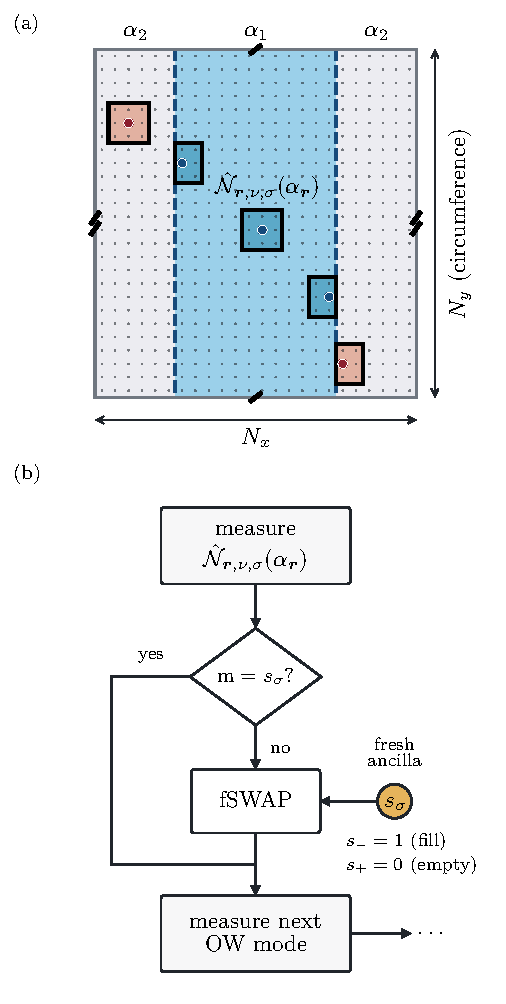
\includegraphics[width=\linewidth,height=148mm,keepaspectratio]{figures/Figure_01_schematic.pdf}
\end{column}\begin{column}{.42\textwidth}
{\color{muted}\fontsize{10}{13}\selectfont Manuscript p.\ 4\hfill\hyperlink{overview}{Overview}\par}\vspace{4mm}
\fontsize{12}{16}\selectfont\raggedright (a) Periodic geometry with $\alpha_{\boldsymbol r}=\alpha_1$ in the central slab and $\alpha_2$ in the trivial exterior. Matching marks identify opposite boundaries. Salmon and blue windows show exterior and slab OW supports; dots mark their centers. Bulk supports contain $3\times3$ cells; interface supports are clipped and renormalized. (b) An occupation measurement returns the Born outcome $\mathrm m$. If $\mathrm m=s_\sigma$, correction is bypassed; otherwise an fSWAP with a fresh ancilla restores $s_-=1$ or $s_+=0$. The branches rejoin and the procedure repeats for subsequent OW modes.
\end{column}\end{columns}\end{frame}
\begin{frame}[label=fig2]{Figure 2\enspace |\enspace Bulk topology in the domain-wall geometry}
\begin{columns}[c,onlytextwidth]\begin{column}{.55\textwidth}\centering
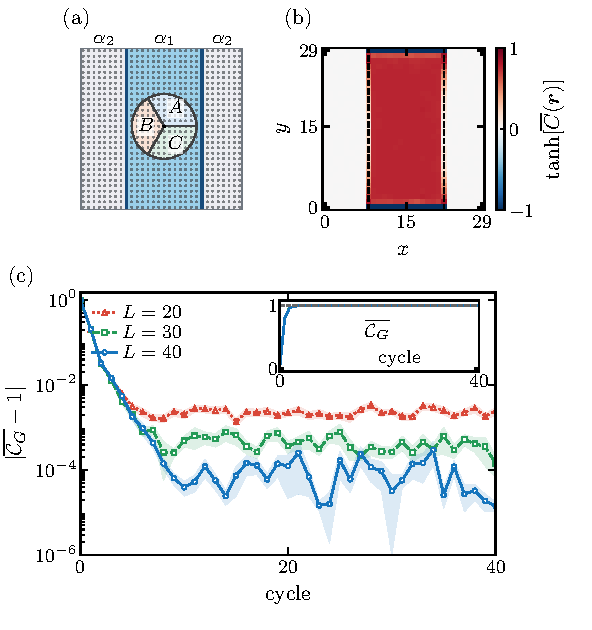
\includegraphics[width=\linewidth,height=148mm,keepaspectratio]{figures/Figure_03_bulk_topology.pdf}
\end{column}\begin{column}{.42\textwidth}
{\color{muted}\fontsize{10}{13}\selectfont Manuscript p.\ 7\hfill\hyperlink{overview}{Overview}\par}\vspace{4mm}
\fontsize{12}{16}\selectfont\raggedright (a) A $30\times30$ lattice with interfaces at $x=8,22$ and a three-sector disk of radius $R=6$. The drawn transverse center is representative. (b) Local Chern marker [Eq.~(11)] at $L=30$, cycle 40, displayed as $\tanh[\overline{C}(\bfr)]$ after averaging $S=100$ independent trajectories. The bounded color scale compresses the periodic-coordinate seam contribution. (c) $|\overline{\mc C_G}-1|$ for $L=20,30,40$, with the untransformed $\overline{\mc C_G}$ in the inset. Each cycle averages ten randomly chosen disk centers per trajectory, then $S=100$ independent trajectories. Shading is one trajectory SEM. All ensembles start from random pure half-filled states and use $\alpha_1=1$, $\alpha_2=30$, and $w=1$.
\end{column}\end{columns}\end{frame}
\begin{frame}[label=fig3]{Figure 3\enspace |\enspace Topological and trivial purification}
\begin{columns}[c,onlytextwidth]\begin{column}{.55\textwidth}\centering
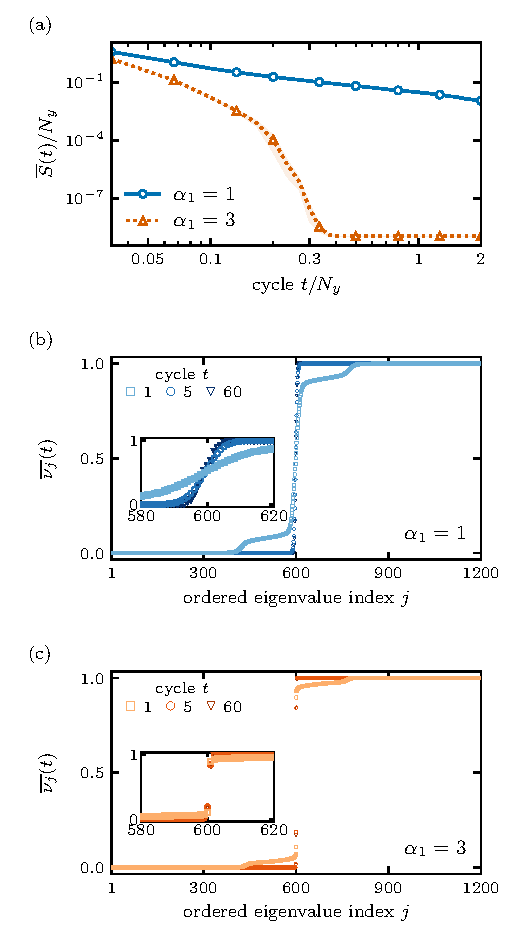
\includegraphics[width=\linewidth,height=148mm,keepaspectratio]{figures/Figure_04_purification.pdf}
\end{column}\begin{column}{.42\textwidth}
{\color{muted}\fontsize{10}{13}\selectfont Manuscript p.\ 8\hfill\hyperlink{overview}{Overview}\par}\vspace{4mm}
\fontsize{12}{16}\selectfont\raggedright Full-system maximally mixed initial states on a $20\times30$ lattice, evolved for 60 cycles with $S=100$ independent trajectories per $\alpha_1$. (a) Mean entropy per circumference for $\alpha_1=1,3$; bands are one trajectory SEM. The trivial plateau is a numerical floor. (b,c) Mean ascending occupation spectra at $t=1,5,60$ for (b) $\alpha_1=1$ and (c) $\alpha_1=3$. Eigenvalues are sorted within each trajectory and cycle before averaging at fixed rank; all 1,200 ranks are displayed as markers. Increasing cycle number runs from light to dark blue in (b) and orange-red in (c), with the same marker shapes in both panels. Insets show ranks $580\leq j\leq620$ with identical limits. Intermediate occupations persist longer in the topological case. For $\alpha_1=3$, covariance eigenvalues are numerically clipped after cycle 30; the endpoint retains this stabilization.
\end{column}\end{columns}\end{frame}
\begin{frame}[label=fig4]{Figure 4\enspace |\enspace Finite-time Lyapunov gap and boundary localization}
\begin{columns}[c,onlytextwidth]\begin{column}{.55\textwidth}\centering
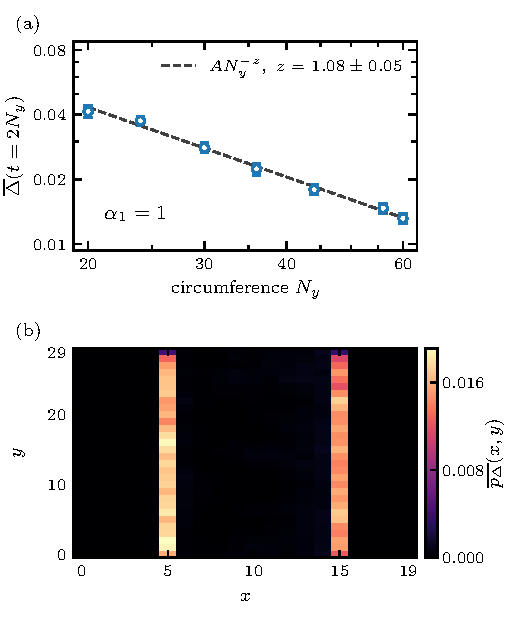
\includegraphics[width=\linewidth,height=148mm,keepaspectratio]{figures/Figure_04_lyapunov.pdf}
\end{column}\begin{column}{.42\textwidth}
{\color{muted}\fontsize{10}{13}\selectfont Manuscript p.\ 9\hfill\hyperlink{overview}{Overview}\par}\vspace{4mm}
\fontsize{12}{16}\selectfont\raggedright (a) Mean gap $\overline{\Delta}(t=2N_y)$ for $\alpha_1=1$ and $N_y=20,24,30,36,44,56,60$ at fixed $N_x=20$. The dashed line is an SEM-weighted fit over all seven sizes, with $z=1.08\pm0.05$; error bars are one trajectory SEM. The slab is initially maximally mixed and the decoupled exterior is pure. (b) Mean spatial density of the unique slowest mode for $\alpha_1=1$, $N_y=30$, and $t=60$, starting with the full system maximally mixed. Each panel uses $S=100$ independent trajectories; gaps and normalized mode densities are evaluated per trajectory before averaging.
\end{column}\end{columns}\end{frame}
\begin{frame}[label=fig5]{Figure 5\enspace |\enspace Algebraic correlation scaling}
\begin{columns}[c,onlytextwidth]\begin{column}{.55\textwidth}\centering
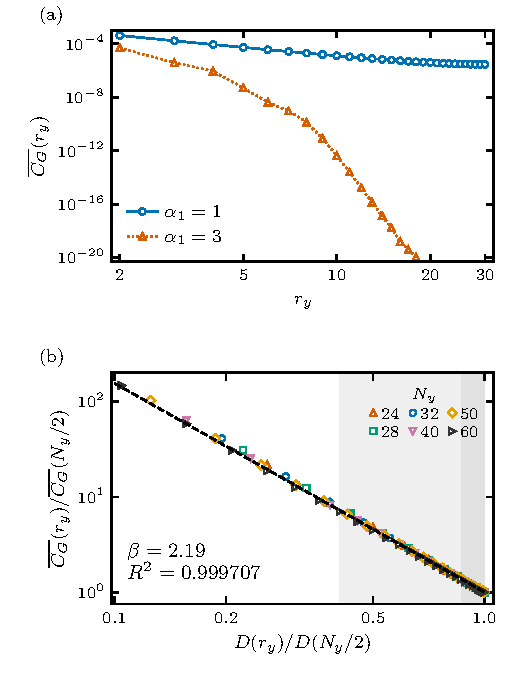
\includegraphics[width=\linewidth,height=148mm,keepaspectratio]{figures/Figure_05_correlations.pdf}
\end{column}\begin{column}{.42\textwidth}
{\color{muted}\fontsize{10}{13}\selectfont Manuscript p.\ 9\hfill\hyperlink{overview}{Overview}\par}\vspace{4mm}
\fontsize{12}{16}\selectfont\raggedright (a) $\overline{C_G}(r_y)$ versus separation $r_y$ at $N_y=60$ for $\alpha_1=1$ (circles, solid) and $3$ (triangles, dotted); values at or below $10^{-20}$ are omitted. (b) Antipodally normalized correlations at $\alpha_1=1$ for $N_y=24,28,32,40,50,60$, plotted against the normalized chord length. Both panels use logarithmic axes and display only $r_y\geq2$. The dashed line is the joint power-law fit over $8\leq r_y\leq N_y/2$, with equal total weight per size and $\beta\approx2.19$; light and darker gray mark the union and overlap of the size-dependent fit windows. Each ensemble contains $S=100$ independent random-pure half-filled trajectories observed after $2N_y$ cycles, with $N_x=20$, $\alpha_2=30$, and $w=1$. The squared correlator is averaged over position and trajectories before the normalization in (b).
\end{column}\end{columns}\end{frame}
\begin{frame}[label=fig6]{Figure 6\enspace |\enspace Entanglement and charge fluctuations}
\begin{columns}[c,onlytextwidth]\begin{column}{.55\textwidth}\centering
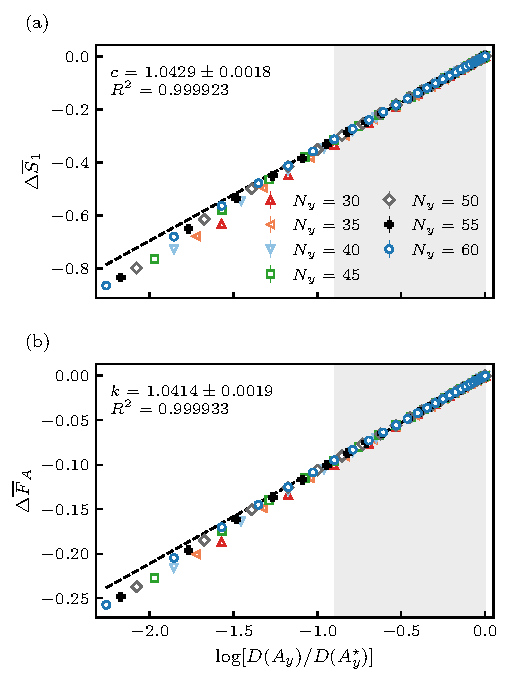
\includegraphics[width=\linewidth,height=148mm,keepaspectratio]{figures/Figure_06_entropy_charge.pdf}
\end{column}\begin{column}{.42\textwidth}
{\color{muted}\fontsize{10}{13}\selectfont Manuscript p.\ 10\hfill\hyperlink{overview}{Overview}\par}\vspace{4mm}
\fontsize{12}{16}\selectfont\raggedright (a) Mean strip entropy and (b) charge variance for $N_y=30,35,\ldots,60$, shifted by their values at $A_y=\lfloor N_y/2\rfloor$. Each case uses $S=100$ independent random-pure half-filled trajectories after $2N_y$ cycles, with all strip origins averaged within each trajectory. Dashed lines are joint fits to Eq.~(23) over $8\leq A_y\leq\lfloor N_y/2\rfloor$ (shaded). The point $A_y=1$ is excluded from display only. The fits and their trajectory-based uncertainties retain correlations between strip widths.
\end{column}\end{columns}\end{frame}
\begin{frame}[label=fig7]{Figure 7\enspace |\enspace Restricted spectra and mode count}
\begin{columns}[c,onlytextwidth]\begin{column}{.55\textwidth}\centering
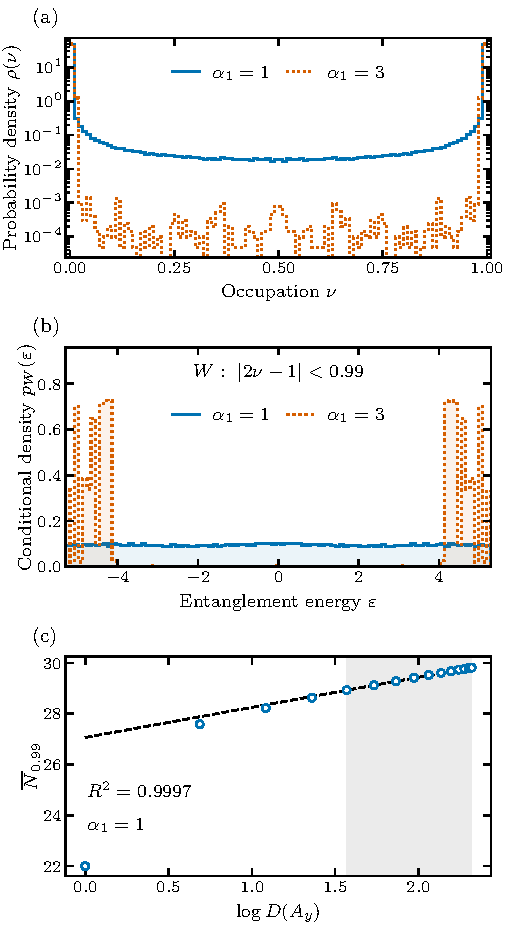
\includegraphics[width=\linewidth,height=148mm,keepaspectratio]{figures/Figure_07_entanglement_spectrum.pdf}
\end{column}\begin{column}{.42\textwidth}
{\color{muted}\fontsize{10}{13}\selectfont Manuscript p.\ 11\hfill\hyperlink{overview}{Overview}\par}\vspace{4mm}
\fontsize{12}{16}\selectfont\raggedright Hard-wall states at $N_x=20$, $N_y=32$, cycle 64, from $S=100$ independent random-pure half-filled trajectories per $\alpha_1=1,3$. (a) Full occupation histogram on $0\leq\nu\leq1$, normalized to unit area. (b) Conditional unit-area energy density for $|2\nu-1|<0.99$, in 101 equal bins on $[-\log199,\log199]$. The central depletion at $\alpha_1=3$ contrasts with the finite near-zero density at $\alpha_1=1$. Both histograms pool all 32 translated half-strips per trajectory. The retained totals are 95,398 and 83,326 for $\alpha_1=1,3$. (c) Raw mean window count for $\alpha_1=1$, averaging origins within each trajectory. Bars are one trajectory SEM; the dashed fit uses $5\leq A_y\leq16$ (shaded), while all widths are displayed.
\end{column}\end{columns}\end{frame}
\begin{frame}[label=fig8]{Figure 8\enspace |\enspace Entropy carried by each wall}
\begin{columns}[c,onlytextwidth]\begin{column}{.55\textwidth}\centering
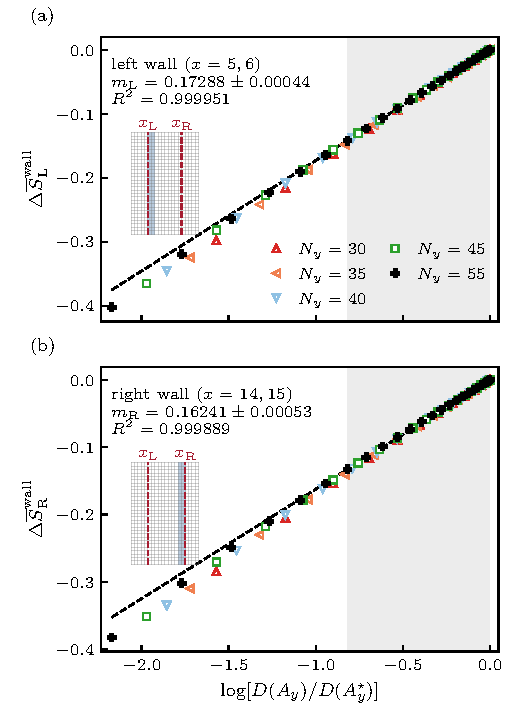
\includegraphics[width=\linewidth,height=148mm,keepaspectratio]{figures/Figure_09_wall_entropy.pdf}
\end{column}\begin{column}{.42\textwidth}
{\color{muted}\fontsize{10}{13}\selectfont Manuscript p.\ 12\hfill\hyperlink{overview}{Overview}\par}\vspace{4mm}
\fontsize{12}{16}\selectfont\raggedright Entanglement contour integrated over (a) $x=5,6$ and (b) $x=14,15$, for $N_y=30,35,40,45,55$. Each case uses $S=100$ independent random-pure trajectories after $2N_y$ cycles. Contours are averaged over all translated strips within each trajectory before trajectory averaging, and anchored at $A_y=\lfloor N_y/2\rfloor$. Dashed lines are joint fits over $8\leq A_y\leq\lfloor N_y/2\rfloor$ (shaded), with equal total weight per size and trajectory-based uncertainties including correlations between widths. Insets mark the integrated columns. The point $A_y=1$ is omitted from display only.
\end{column}\end{columns}\end{frame}
\begin{frame}[label=fig9]{Figure 9\enspace |\enspace Modular evolution on the walls}
\begin{columns}[c,onlytextwidth]\begin{column}{.55\textwidth}\centering
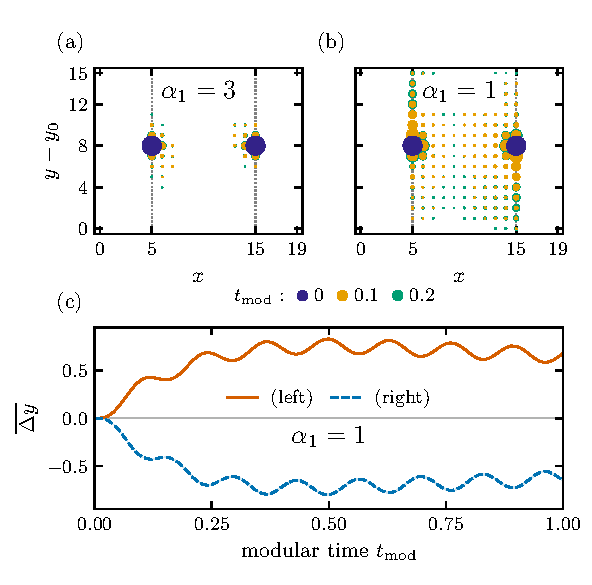
\includegraphics[width=\linewidth,height=148mm,keepaspectratio]{figures/Figure_10_modular_evolution.pdf}
\end{column}\begin{column}{.42\textwidth}
{\color{muted}\fontsize{10}{13}\selectfont Manuscript p.\ 13\hfill\hyperlink{overview}{Overview}\par}\vspace{4mm}
\fontsize{12}{16}\selectfont\raggedright Two incoherent orbital profiles are initialized at each source cell $(x,\delta y)=(5,A_y/2)$ or $(15,A_y/2)$ in a half-cylinder of $A_y=16$ rows. The states come from $S=100$ independent random-pure trajectories per $\alpha_1=1,3$ on a $20\times32$ lattice after 64 cycles. (a,b) Mean densities at $t_{\rm mod}=0,0.1,0.2$ (purple, orange, green) for (a) $\alpha_1=3$ and (b) $\alpha_1=1$. (c) Mean center-of-mass displacement $\overline{\Delta y_{x_s}}$ from the initial row $\delta y=A_y/2$, defined in Eq.~(36), for $\alpha_1=1$. Solid (left) and dashed (right) lines denote $x_s=5$ and $15$; each five-column window is normalized by its retained weight before averaging. Each observable is evaluated per cut, then averaged over 32 origins and trajectories. Bands are one trajectory SEM. Centered occupations are clipped at $\pm(1-10^{-10})$ when constructing $h_A$.
\end{column}\end{columns}\end{frame}
\begin{frame}[label=fig10]{Figure 10\enspace |\enspace Trajectory-averaged dynamics and channel gap}
\begin{columns}[c,onlytextwidth]\begin{column}{.55\textwidth}\centering
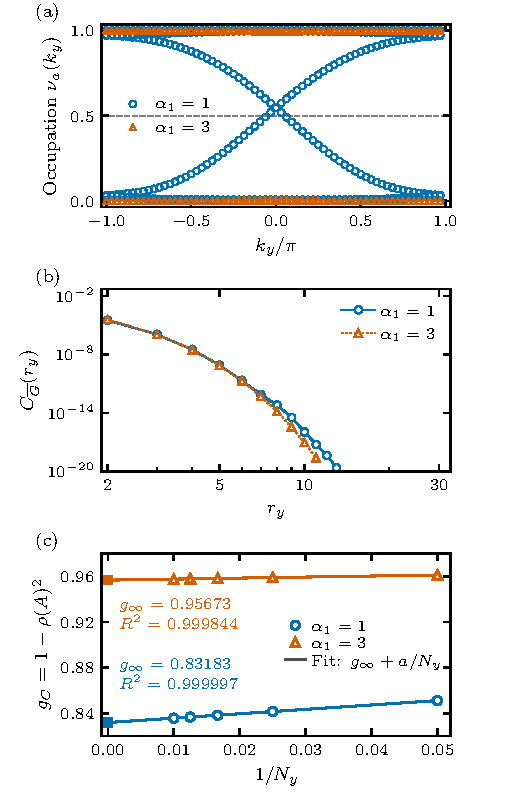
\includegraphics[width=\linewidth,height=148mm,keepaspectratio]{figures/Figure_11_mean_channel.pdf}
\end{column}\begin{column}{.42\textwidth}
{\color{muted}\fontsize{10}{13}\selectfont Manuscript p.\ 14\hfill\hyperlink{overview}{Overview}\par}\vspace{4mm}
\fontsize{12}{16}\selectfont\raggedright (a) Occupations of the translation-averaged two-point matrix and (b) its squared correlation at $N_y=64$, after 128 cycles from maximal mixing, for $\alpha_1=1,3$. Panel (b) uses logarithmic axes for $C_{\overline G}(r_y)$ versus $r_y\geq2$; correlations below $10^{-20}$ are not displayed. (c) Fits of the multiplier gap $g_C=1-\rho(A)^2$ to $g_\infty+a/N_y$ at $\alpha_1=1,3$, with fixed $N_x=20$ and all five sizes $N_y=20,40,60,80,100$; squares at $1/N_y=0$ mark extrapolated intercepts. Outcomes are averaged analytically in the fixed repeated raster schedule, so there is no sampled-trajectory count or SEM.
\end{column}\end{columns}\end{frame}
\begin{frame}[label=figA1]{Figure A1\enspace |\enspace Truncated OW modes at $\alpha=1$}
\begin{columns}[c,onlytextwidth]\begin{column}{.55\textwidth}\centering
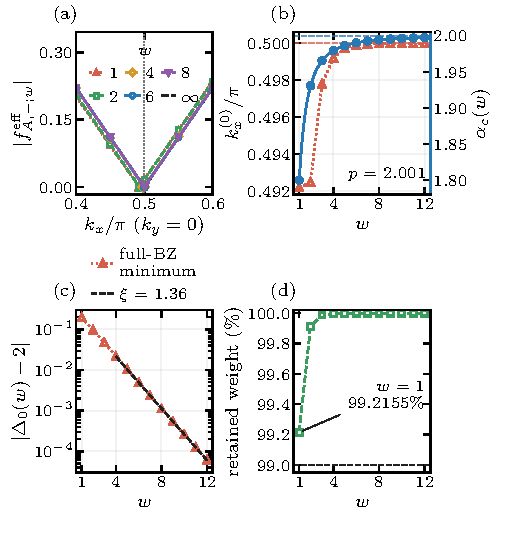
\includegraphics[width=\linewidth,height=148mm,keepaspectratio]{figures/Figure_A01_ow_truncation.pdf}
\end{column}\begin{column}{.42\textwidth}
{\color{muted}\fontsize{10}{13}\selectfont Manuscript p.\ 16\hfill\hyperlink{overview}{Overview}\par}\vspace{4mm}
\fontsize{12}{16}\selectfont\raggedright (a) Effective form factor $|f^{\rm eff}_{A,-;w}|$ along $k_y=0$ for $w=1,2,4,6,8,\infty$. Symbols mark the zeros, and the dotted line marks the untruncated zero. (b) Position of the winding-$(-1)$ zero (red, left axis) and the critical parameter $\alpha_c(w)$ of the truncated parent Hamiltonian (blue, right axis) with the fit of Eq.~(A11). Dashed lines mark the $w=\infty$ values. (c) Deviation of the half-filling gap $\Delta_0(w)$ of the truncated parent Hamiltonian from its untruncated value, with an exponential fit for $w\geq4$. (d) Fraction of the squared OW norm retained inside the window.
\end{column}\end{columns}\end{frame}
\begin{frame}[label=figA2]{Figure A2\enspace |\enspace Spatial entanglement and antipodal mutual information}
\begin{columns}[c,onlytextwidth]\begin{column}{.55\textwidth}\centering
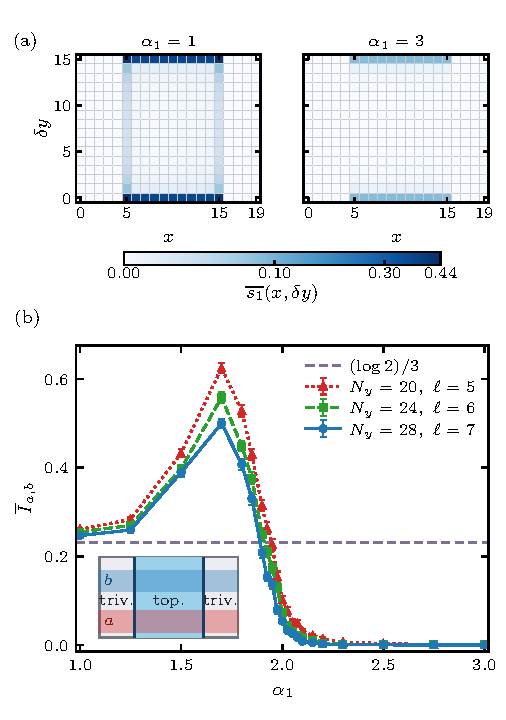
\includegraphics[width=\linewidth,height=148mm,keepaspectratio]{figures/Figure_A02_mutual_information.pdf}
\end{column}\begin{column}{.42\textwidth}
{\color{muted}\fontsize{10}{13}\selectfont Manuscript p.\ 19\hfill\hyperlink{overview}{Overview}\par}\vspace{4mm}
\fontsize{12}{16}\selectfont\raggedright (a) Mean entropy contours for $\alpha_1=1,3$ on a $20\times32$ lattice, for half-strips of 16 rows at cycle 64. All 32 strip origins are averaged within each of $S=100$ independent random-pure trajectories before averaging trajectories. The shared colorbar uses a square-root scale; $\delta y$ is relative to the strip origin. (b) Mean mutual information of antipodal full-width strips with $\ell=N_y/4$, for $N_y=20,24,28$ after $2N_y$ cycles. Each parameter uses a separate set of $S=100$ random-pure trajectories; all distinct strip translations are averaged first. Bars are one trajectory SEM. The dashed line is $(\log2)/3$, and the inset shows the strip geometry. Both panels use hard walls and $w=1$; their ensembles are distinct.
\end{column}\end{columns}\end{frame}
\begin{frame}[label=figA3]{Figure A3\enspace |\enspace Convergence of the entropy coefficient}
\begin{columns}[c,onlytextwidth]\begin{column}{.55\textwidth}\centering
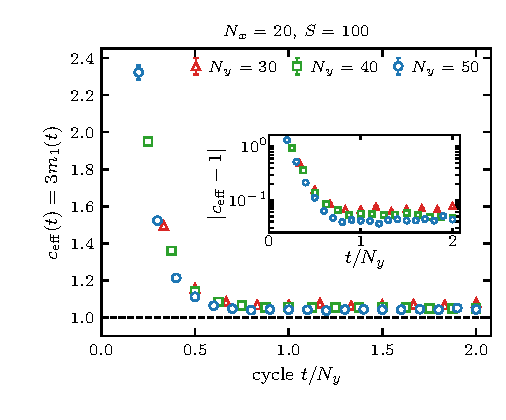
\includegraphics[width=\linewidth,height=148mm,keepaspectratio]{figures/Figure_08_central_charge.pdf}
\end{column}\begin{column}{.42\textwidth}
{\color{muted}\fontsize{10}{13}\selectfont Manuscript p.\ 20\hfill\hyperlink{overview}{Overview}\par}\vspace{4mm}
\fontsize{12}{16}\selectfont\raggedright Cycle dependence of $c_{\rm eff}=3m_1$ for $N_x=20$ and $N_y=30,40,50$, from $S=100$ independent random-pure trajectories per size evolved through $2N_y$ cycles. Strip origins are averaged within each trajectory, then trajectories are averaged before fitting $\overline S$ versus log chord length with a free intercept over $8\leq A_y\leq N_y/2$. Points show every fifth cycle from $t=10$; bars are three times the regression standard error of the mean-curve slope. The inset resolves $|c_{\rm eff}-1|$ on a logarithmic scale. The dashed horizontal reference is one.
\end{column}\end{columns}\end{frame}
\begin{frame}[label=figA4]{Figure A4\enspace |\enspace Parameter dependence of the averaged-channel gap}
\begin{columns}[c,onlytextwidth]\begin{column}{.55\textwidth}\centering
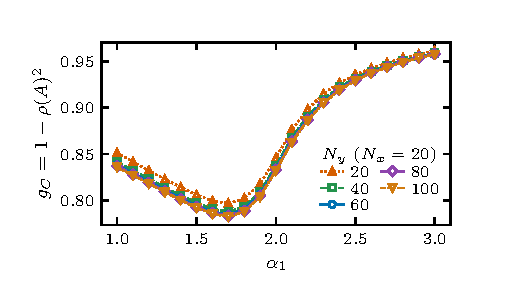
\includegraphics[width=\linewidth,height=148mm,keepaspectratio]{figures/Figure_A04_channel_gap_scan.pdf}
\end{column}\begin{column}{.42\textwidth}
{\color{muted}\fontsize{10}{13}\selectfont Manuscript p.\ 23\hfill\hyperlink{overview}{Overview}\par}\vspace{4mm}
\fontsize{12}{16}\selectfont\raggedright Exact multiplier gap $g_C=1-\rho(A)^2$ for the fixed raster schedule at $N_x=20$ and $N_y=20,40,60,80,100$. Each size uses 21 equally spaced values of $\alpha_1$ from 1 to 3, with $\alpha_2=30$ and hard-wall OW range $w=1$. These are deterministic one-cycle spectral calculations, with no sampled trajectories or statistical error bars. Lines connect sampled points as guides to the eye.
\end{column}\end{columns}\end{frame}
\end{document}
